\section{Empirical determination of radius of curvature for a bow shock of unknown orientation}
\label{app:rcurv-empirical}


\begin{figure*}
  \centering
  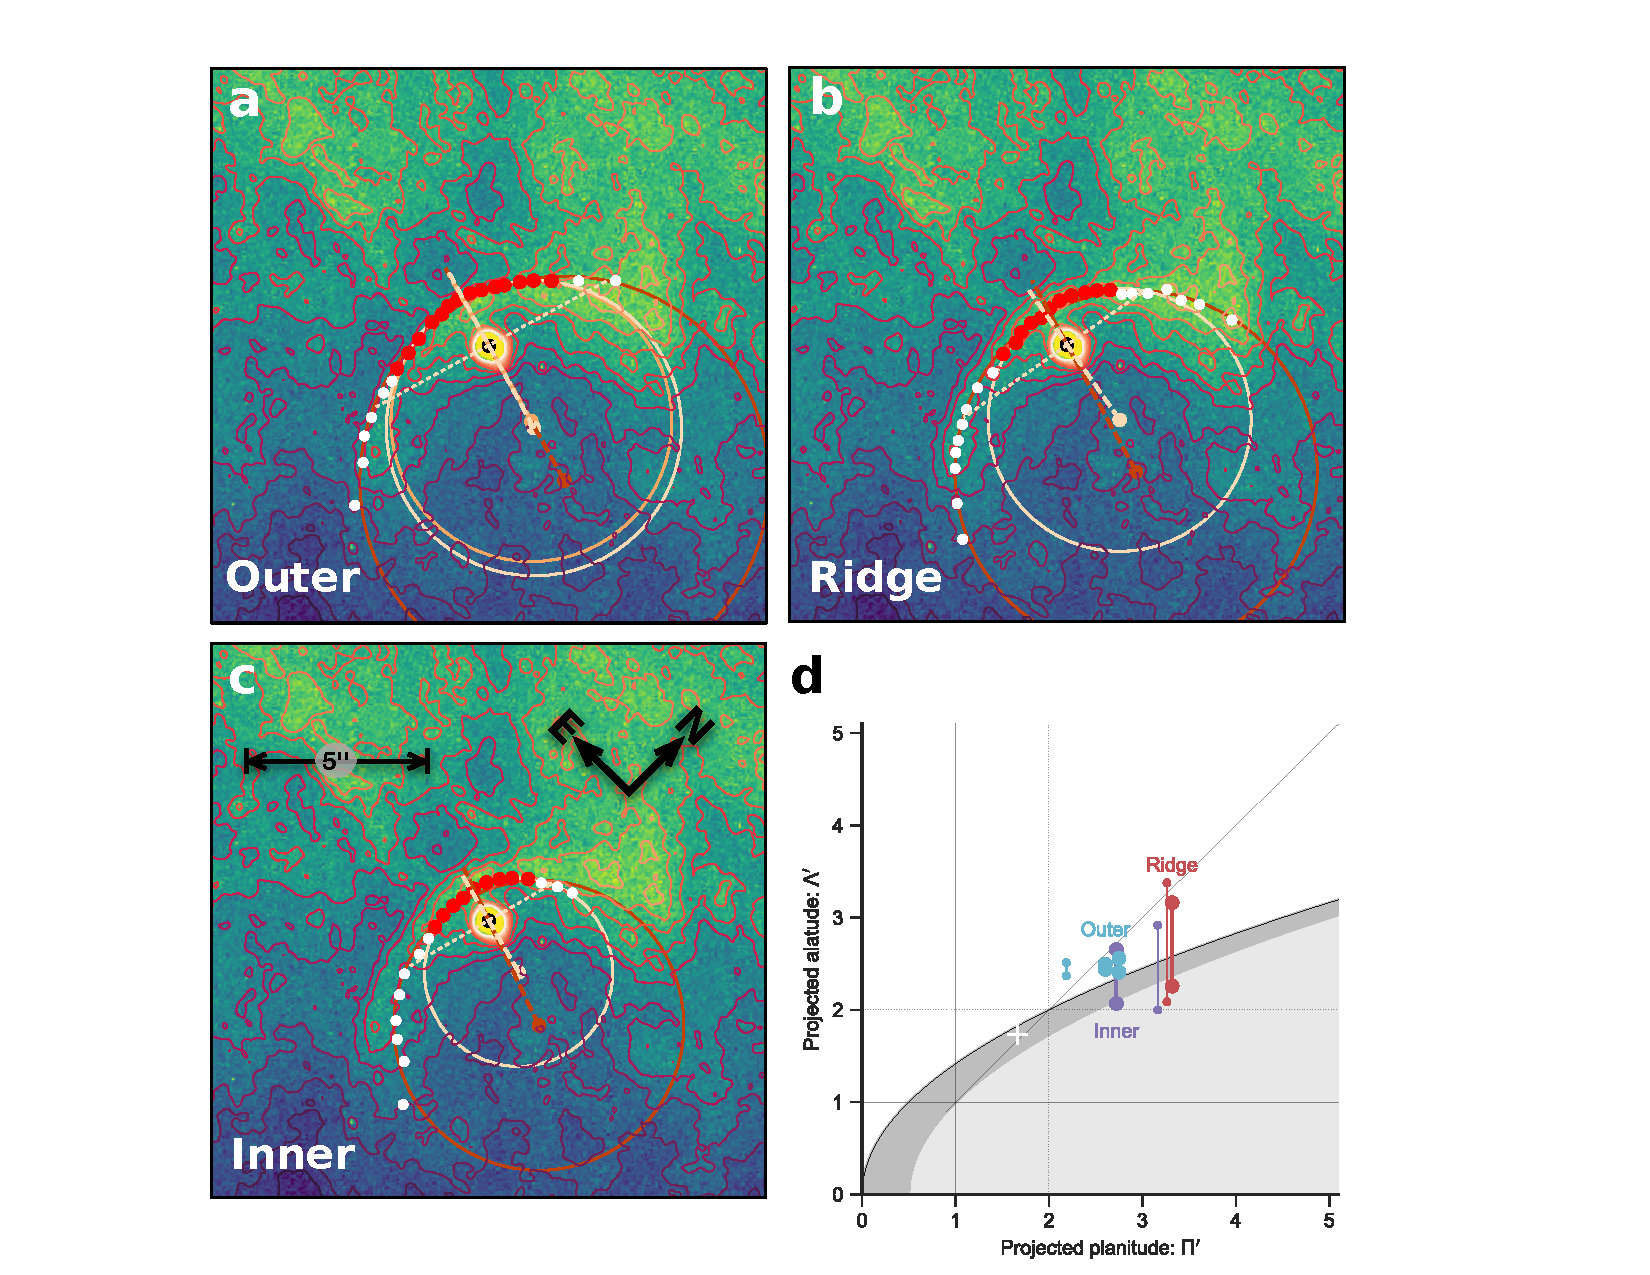
\includegraphics[width=\linewidth]{figs/new-000-400-multi-fig}
  \caption{Example empirical determination of planitude and alatude
    for an observed bow shock}
  \label{fig:000-400-fit}
\end{figure*}

Consider a set of \(N\) points on the plane of the sky, with Cartesian
coordinates \(\bm{r}_k = (x_k, y_k)\) for \(k = 1 \dots N\).  We wish
to estimate the radius of curvature of the smooth curve that the set
of points is presumed to be sampled from.  To do this, we fit a circle
to the points as follows.  The circle is defined by its center,
\(\bm{r}_{\C} = (x_{\C}, y_{\C})\), and radius, \(R_{\C}\).  For a
given circle, we define a mean radius of the set of points from the
circle center:
\begin{equation}
  \label{eq:rcurv-mean-radius}
  \bar{R}(x_{\C}, y_{\C}) = \frac{1}{N}  \sum_{k = 1}^{N} \Abs{\bm{r}_k - \bm{r}_{\C}}  \ .
\end{equation}
We then optimize\footnote{%
  For example, using a Levenberg-Marquardt algorithm, such as
  \texttt{astropy.modeling.fitting.LevMarLSQFitter} from the AstroPy
  library \citep{Astropy-Collaboration:2013a}.} %
to find best-fit values \((x_{\C}^*, y_{\C}^*)\), which minimize the
objective function
\begin{equation}
  \label{eq:rcurv-objective-function}
  f(x_{\C}, y_{\C}) = \sum_{k = 1}^{N} \left(
    \abs{\bm{r}_k - \bm{r}_{\C}}  - \bar{R} (x_{\C}, y_{\C}) \right)^2 \ .
\end{equation}
The best-fit radius of curvature is then given by
\(R_{\C}^* = \bar{R}(x_{\C}^*, y_{\C}^*)\).

If we also know the position, \(\bm{r}_0 = (x_0, y_0)\), of the bow's
central source, then we can find the unit vector in the direction of
the bow's projected axis as
\begin{equation}
  \label{eq:rcurv-axis-vector}
  \uvec{\xi} = \frac {\bm{r}_0 - \bm{r}_{\C}^*} { \abs{\bm{r}_0 - \bm{r}_{\C}^*}} \ , 
\end{equation}
and the apex distance from the source as\footnote{%
  This is only valid if the resultant \(R_0 < R_{\C}^*\), otherwise
  the opposite sign of \(\uvec{\xi}\) must be taken.}
\begin{equation}
  \label{eq:rcurv-apex-distance}
  R_0 = \Abs{\bm{r}_{\C}^* + R_{\C}^* \uvec{\xi} - \bm{r}_0} \ .
\end{equation}
A refinement of the method is then to repeat the circle fit after
restricting the set of points to those lying within a certain angle
\(\Delta\theta\) of the bow axis by requiring
\begin{equation}
  \label{eq:rcurv-delta-theta}
  \uvec{\xi} \cdot 
  {\left( \bm{r}_k - \bm{r}_{\C}^* \right) }
  \ge   {\Abs{\bm{r}_k - \bm{r}_{\C}^*}}
  \cos \Delta\theta \ ,
\end{equation}
where we find that best results are obtained with \(\Delta\theta \le \ang{30}\).

If quantitative estimates exist for the uncertainties, \(\epsilon_k\), in the
measurements of \(\bm{r}_k\), then it is appropriate to incorporate
weights of \(\epsilon_k^{-2}\) in the objective function.  In cases where the
bow shape is traced by eye, based on real or synthetic observations, a
more practical approach is to maintain uniform weighting but to place
a greater density of points \(\bm{r}_k\) in regions where the shape is
well-determined and to place them more sparsely in regions where the
shape is less certain.

Note that this method is not necessary if the orientation of the bow
axis is known a~priori, in which case the Taylor series method
described in \S~\ref{sec:plan-alat-bow} is more efficient and
accurate.

%%% Local Variables:
%%% mode: latex
%%% TeX-master: "quadrics-bowshock"
%%% End:
